In the last chapter, we saw the theoretical foundation on NLP techniques. In this chapter, we will review in the literature some works that use the NLP techniques described to discover topics in a data set. In addition, we will show some applications for this type of task. And, finally, some final remarks to continue this work.


\section{Topics Discovery}

Finding meaningful topics in a document collection has been used for a lot of authors for the most various applications. For example, \citeonline{hurtado2016topic} use topic modeling to inspect research publications, patents, and technical reports aiming to model the evolution of the direction of research and forecast the near future trends in IT industry.

Using the titles and abstracts of a data set with more than six thousand academic papers between 2002 and 2010, mostly collected by \citeonline{tang2008arnetminer}, they proposed a sentence-level association rule to discover the meaningful topics. After categorizing the documents in topics, they were capable of building time series for each found topic, marking how many times that topic was cited in a given year. So, they were able to build an ensemble of forecasters to study the patterns and relationships among topics over the years.

For a better understanding, the Figure \ref{fig:topic-discovery-framework} has a flowchart with their proposed framework for the topic discovery and forecasting.

\begin{figure}[h!]
	\centering
	
\includegraphics[width=0.6\linewidth]{01.Chapters/03.RelatedWorks/topic-discovery-framework}
	\caption{Flowchart of the proposed framework \cite{hurtado2016topic}.}
	\label{fig:topic-discovery-framework}
\end{figure}

This framework involves some well-known major steps of NLP processing. First, they convert the documents into a transactional form, i.e., the phrases in each document will be considered individually during the process. Next, they perform the basic normalization steps which includes case conversion, tokenization, removing step words, part of speech tagging, stemming and lemmatization. It is also performed an additional step, specific to their application, removing verbs such as ``exploiting'', ``adapting'' and ``propose'', because they are very common in scientific publications and do not add much meaningful information.

To vectorize the transactions, it is used a slight variation of BoW. Instead of word counting, it is only checked whether a word belongs to a transaction, this is called the binary incidence matrix. The topic discovery step comes afterwards, applying an association rule mining to the transactions and discovery their patterns. In order to avoid different topics with redundant words, is applied a rule refinement process that allows similar topics to be combined.

Online forums and social media are excellent platforms for people discuss and share information about the most kind of subjects. Recently, the topic discovery technique was used to summarize different topics related to COVID-19 disease and perform a sentiment analysis on them~\cite{jelodar2020deep}.

Reddit is a discussion website in which its users can submit posts and start discussions with other community members. The posts are organized in the called ``sub reddits'', boards created by users to discuss a specific subject. Using over half million comments from 10 health related sub reddits with information about COVID-19, \citeonline{jelodar2020deep} performed a topic discovery to group similar comments. So, applying a sentiment analysis on each comment it was possible to summarize the average opinion about the discovered topics.


\section{Trend Forecast}

Predicting future trends can be very helpful in various applications, like to model the evolution of research. Following the topic discovery process from \citeonline{hurtado2016topic}, a forecast trend was used to predict the near future related to each discovered topic. With all documents belonging to at least one identified topic in the set, was created a topic incidence matrix that contains the count of times a topic is mentioned over the years. Finally, they make a ensemble forecasting to predict the future topic counting using the framework shown in Figure \ref{fig:ensemble-forecasting-framework}.

\begin{figure}[h!]
	\centering
	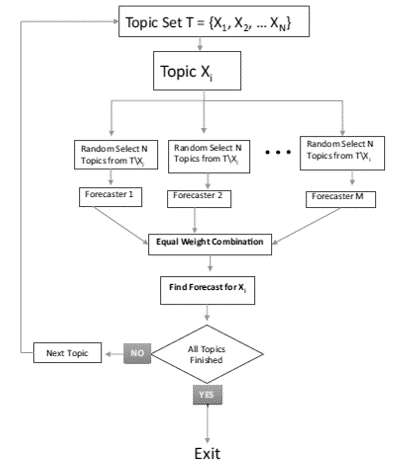
\includegraphics[width=0.5\linewidth]{01.Chapters/03.RelatedWorks/ensemble-forecasting-framework}
	\caption{Ensemble forecaster framework \cite{hurtado2016topic}.}
	\label{fig:ensemble-forecasting-framework}
\end{figure}

Given a specific topic, they generate $M$ forecasters which target $X_{i}$ along with N randomly chosen fields, excluding $X_{i}$. Then, the predicted value, $\hat{X}_{i}(t+1)$, is an average of each individual forecast, $\hat{X}_{i, F_{k}}(t+1)$, calculated by 

\begin{equation}
	\hat{X}_{i}(t+1) = \dfrac{1}{M} \sum_{k=1}^{M}\hat{X}_{i, F_{k}}(t+1)\text{.}
\end{equation}

By evaluating metrics like the coefficient of determination (R-squared) and mean squared error (MSE) they were able to conclude the ideal number $N$ of variables to predict more accurately the future for all topics in the set.

\citeonline{shentopic} also predicted trends by analyzing the exponential growth in the volume of scholarly articles published over the years. However, he skips the NLP process step by using a pre-labeled data set from Springer containing the number of works above 14 subjects in 25 years. Using ensemble forecast based on neural networks and support vector regression he was able to study the topics growth and codependency between them.


\section{Final Remarks}

